\documentclass[12pt,english]{amsart}
\usepackage{amssymb,amsmath,amscd,graphicx,fontenc,bbold,amsthm,mathrsfs,mathtools}
\usepackage[pdftex,bookmarks,colorlinks,breaklinks]{hyperref}
\usepackage{comment}
\usepackage{graphicx}
\usepackage[top=3cm,bottom=3cm,right=2.3cm,left=2.3cm,twoside=false]{geometry}

\hypersetup{linkcolor=blue,citecolor=red,filecolor=dullmagenta,urlcolor=blue}
%\usepackage{verbatim}
%\usepackage{showkeys}

\newtheorem{theorem}{Theorem}[section]
\newtheorem{definition}{Definition}
\newtheorem{lemma}[theorem]{Lemma}
\newtheorem{proposition}[theorem]{Proposition}
\newtheorem{corollary}[theorem]{Corollary}
\theoremstyle{definition}
\newtheorem{remark}{Remark}
\newtheorem{conj}{Conjecture}
\newtheorem{notation}{Notation}

\DeclarePairedDelimiter\abs{\lvert}{\rvert}%
\DeclarePairedDelimiter\norm{\lVert}{\rVert}%
\newcommand{\snxk}{\pi(x,k)}
\newcommand{\bnxk}{{\mathrm{N}}(x,k)}
\newcommand{\px}[1]{\pi(x,{#1})}
\newcommand{\Px}[1]{\Pi(x,{#1})}

\graphicspath{ {./img/} }

\title{Wasserstein Auto-Encoders}
\author{Marzieh Mehdizadeh, Joseph D Viviano, Johnathan Guymont}
\address{ D\'epartement d'informatique et de recherche op\'erationnelle
          Universit\'e de Montr\'eal
          Pavillon Andr\'e-Aisenstadt, DIRO.}
\date{April 2018}
%\linespread{1.15}

\begin{document}

\maketitle
%\tableofcontents
%==========================================

\section{Paper Summary}
\subsection{Motivation}
(What is the problem)\\
In this paper,the authors introduce a new efficient algorithm called Wasserstein
Auto-Encoders (WAE) to build a generative model of data distribution. This
generative model is based on the optimal transport (OT) finding the minimum
Wasserstein distance between the true data probability distribution (unknown
distribution) $P_X$ and the latent variable distribution $P_G$. In other words,
WAE minimizes a penalized form of the Wasserstein distance between $P_X$ and
$P_G$ which leads to a regularizer that is different form the regularizer in
VAE. This regularizer helps the posterior $P_G(X|Z)$ distribution of data points
$X\in \mathcal{X}$ to match the prior $P_Z$ of latent codes $Z \in \mathcal{Z}$.

\subsection{Proposed approach}

(Analysis)\\

First we list the main contributions of this paper as below:

\begin{enumerate}
  \item The first and the main contribution is the family of Wasserstein
        Auto-Encoders (WAE) defined as above. The loss function of WAE algorithm
        is a combination of two following important terms:

$$\text{Loss= reconstruction cost+ a regularizer penalizng a discrepancy between distributions}$$
The cost function is the squared cost and the regularizer is denoted as
$D_{Z}(P_Z, Q_Z)$ , where $Q_Z$ is the distribution of encoded data points
defined by $Q_Z:= \mathbb{E}_{P_X} \left[Q(Z|X) \right]$.

  \item We use two MNIST and CelebA datasets to evaluate the WAE algorithm and we
        will observe that the generated samples are less blurry than VAE's generated
        samples.

  \item Two different form of regularizer $D_Z(P_Z, Q_Z)$ will be introduced: One
        is based on the adversarial training in latent space $\mathcal{Z}$ (Like
        GANs) so we denote it the \textbf{ GAN-based $\mathcal{D}_Z$} and the
        other form is based on the maximum mean discrepancy denoted as
        \textbf{MMD-based $\mathcal{D}_Z $}

  \item Theoretical part containing a theorem that helps finding objective
        function for WAE.

\end{enumerate}

\textbf{How WAE works:}

The WAE method tries to minimize the optimal transport cost $W_c(P_X, P_G)$ such
the the decoder and encoder have the following tasks:\\

\textbf{Decoder:} It tries to reconstruct the encoded training examples with a
good accuracy by using the cost function c, defined by $c(x,y)= ||x-y||_2^2$.

\textbf{Encoder:} It simultaneously does two tasks: It tries to match the encoded
distribution of training examples $Q_z$ to the prior $P_Z$ measured by using one
of the form of $\mathcal{D}_Z(Q_Z,P_Z)$ introduced above, and at the same time it
makes sure that the latent codes $Z \in \mathcal{Z}$ are learning enough to
reconstruct the encoded training examples.  In \ref{fig:WAE} we give more explanation
that how WAE is more efficient than VAE.

\begin{figure}[h!]
\centering
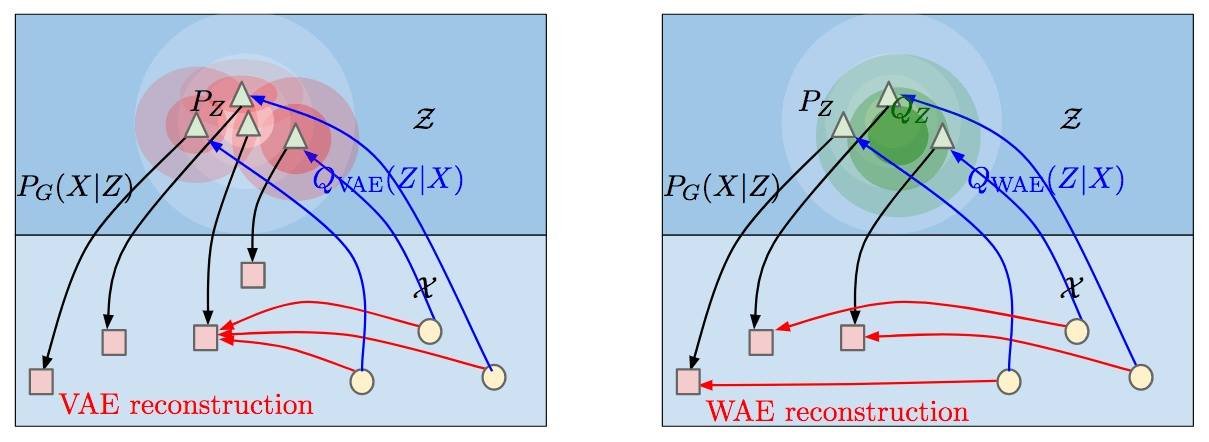
\includegraphics[width=0.9\textwidth]{diagram}

\caption{In these figures circles true data points $X$ for data space
$\mathcal{X}$, triangles are the latent points $Z$ from space $\mathcal{Z}$,
squares represent the generated samples $Y$ and arrows show the different
conditional distributions. In both cases VAE (left) and WAE (right) we have to
minimize the $c(x,y)$ and $\mathcal{D}_Z(P_Z,Q_Z)$  but there is a big
dereference that as we observe in left, VAE tries to encourage every single
$Q(Z|X=x)$ shown by the red balls to match $P_Z$ shown by the white ball, but
the problem is that the red balls have intersection which leads the blurriness
problem to the reconstructed results. On the other hand, WAE forces the
expectation $Q_Z= \mathbb{E}_{P_X}\left[ Q(Z|X)\right]$  with the green balls to
match $P_Z$ shown by white balls. If we define
$\Gamma_{VAE}(Y|X)= P_G(Y|Z)+ Q_{VAE}(Z|X)$ and
$\Gamma _{WAE}(Y|X)= P_G(Y|Z)+ Q_{VAE}(Z|X)$ which are shown by the red arrows,
then we see that in the left picture the data point $X$ are mapped to a same $Y$
with a hight probability while in the right picture data points $X$ are mapped to
$Y$ a lower probability. }

\label{fig:WAE}
\end{figure}\\

 \textbf{What is Wasserstein distance?}
Wasserstein Distance is a measure of the distance between two probability
distributions.( It is also called Earth Mover's distance, short for EM distance,
because informally it can be interpreted as moving piles of dirt that follow one
probability distribution at a minimum cost to follow the other distribution.)
The cost is quantified by the amount of dirt moved times the moving distance. We
take the minimum one among the costs of all dirt moving solutions as the EM
distance. In the definition of Wasserstein distance, the inf (infimum, also
known as greatest lower bound) indicates that we are only interested in the
smallest cost.) More formally we define the Wasserstein distance as follows:

\begin{equation}
\label{eq:ot}
W_c(P_X,P_G):=\inf_{\Gamma\in \mathcal{P}(X\sim P_X,Y\sim P_G)} \mathbb{E}_{(X,Y)\sim\Gamma}[c(X,Y)]\,,
\end{equation}

where $c(x,y)$ is any measurable cost function and
$\mathcal{P}(X\sim P_X,Y\sim P_G)$ is the set of all possible joint probability
distribution between $P_X$ and $P_G$.

\textbf{Why Wasserstein distance is better than JS or KL divergence used in VAE?}

Even when two distributions are located in lower dimensional manifolds without
overlaps, Wasserstein distance can still provide a meaningful and smooth
representation of the distance in-between. Let's give an examples: If $P$ and
$Q$ are two probability distributions and we define:

$$\forall (x,y) \in P, x=0 , y\sim U(0,1)$$
$$\forall (x,y) \in Q, x=\theta, 0\leq \theta \leq 1, y\sim U(0,1)$$
when $\theta \not=0$.\\
$$D_{KL}(P||Q)= \sum _{x=0, y \sim U(01)} 1. \log(1/0)= +\infty,$$
$$D_{KL}(Q||P)= \sum _{x=\theta, y \sim U(01)} 1. \log(1/0)= +\infty,$$
$$D_{Js} (P,Q)= 1/2 \left( \sum_{X=0. y \sim U(0,1)}1. \log \frac{1}{(1/2)}+ \sum_{X=0, Y\sim U(0,1)}1. \log \frac{1}{(1/2)}\right)= \log 2$$

and

$$W(P,Q)= |\theta|$$

But when $\theta=0$, two distributions are fully overlapped:

$$D_{KL}(P||Q)= D_{KL}(Q||P)= D_{JS}(P,Q)=0,$$

and

$$W(P,Q)=0=|\theta|$$

$D_{KL}$ gives us inifity when two distributions are disjoint. The value of
$D_{JS}$ has sudden jump, not differentiable at $\theta=0$. Only Wasserstein
metric provides a smooth measure, which is super helpful for a stable learning
process using gradient descents.

\section{Experiments}

\subsection{Motivation for the experiments}

To evaluate any improvement in learning the latent data distribution using
the optimial transport-based Wasserstien distance over the standard variational
auto encoder approch (making use of the KL-divergence), the authors trained 3
models: a 'stock' VAE, a WAE using the GAN-based Wasserstien penalty, and a WAE
using the MDD-based Wasserstien penalty. The motivation was to empirically test
whether the Wasserstein distance improves the reconstruction quality observed.

\subsection{Reproducing the main results}

The reproduction of this paper can be found in the following repo:\\

\begin{center}\textbf{https://github.com/josephdviviano/wae}\end{center}\\

These experiments were run on both the celeba and mnist datasets. Note that,
due to time restictions, we only trained our models on 10\% of the celeba
dataset, and used a small test set of 1000 images.



    Motivation of the experiments


    What are the authors trying to demonstrate with the experiments?

    Are there experiments that might demonstrate weaknesses/strengths that should be there but arent?

    Are there any flaws in the experiments they run? What are they?

    Reproducing main results (tables, figures, etc)


\section{Discussion}

We are not critical of the experiments conducted considering the nature of the
result. Namely, they present a new kind of generative model, and then compare
the performance of this model using standard generative-model measures on stock
datasets. \\

We are critical that not many quantitative results are shown. Training curves
would have been welcome. There was also very little discussion of training
stability, which we found to be an extremely challenging aspect of this
replication. \\

We found multiple details of the implementation in the official source code
not reported in the paper. All references below refer to the official code: \\

\begin{center}\textbf{https://github.com/tolstikhin/wae}\end{center}\\

\begin{itemize}

    \item{For the reconstruction term of the loss (mean squared error), the
          authors \textbf{scale it by 5\%} (line 335 of wae.py). This is
          obviously crucial, as it weights the reconstruction term of the WAE
          loss (\verb|RECON + LAMBDA * PENALTY|) quite low compared to how they
          present the results in the paper. In our experiments, we tried using
          this scaling factor, lovingly called \verb|SCALEBULLSHIT|.}

    \item{For the MMD loss, the MMD value is accumulated times over different
          scales (line 294 of wae.py). We copied this implementation detail, but
          are unsure of it's relevance. Nonetheless, this implementation detail
          should be covered in the paper, or at the very least, be justified by
          a comment in the code.}

    \item{We found training to be rather unstable for the MMD method in
          particular. Training tended to collapse if the mean or standard
          deviation of the encoded data grew too large, which happened
          frequently for the MMD method. The authors combat this by clamping the
          sigma value during reparameterization between -50 and 50, which they
          do not comment on anywhere in the paper or code. We found this to be a
          crucial implementation detail.}

    \item{}

\bibliographystyle{plain}
\bibliography{references}

\end{document}
